%
% fourierGrundlagen.tex -- Mathematische Grundlagen der Fourier Reihe & Transformation
%
% (c) 2020 Prof Dr Andreas Müller, Hochschule Rapperswil
%
% !TEX root = ../../buch.tex
% !TEX encoding = UTF-8
%

\section{Fourierreihe\label{fourier:section:GrundlagenFourierAnalyse}}
\kopfrechts{Fourierreihe}


Mit der Fourier-Reihe lassen sich periodisch wiederholende Funktionen, wie ein Rechteck- oder Dreiecksignal, mit skalierten Sinus- und Kosinusschwingungen darstellen. 
Um die Reihe aufzustellen, braucht man nur drei Arten von Koeffizienten zu bestimmen. 

\begin{itemize}
	\item $a_0$ ist der Mittelwert, der Funktion. 
	Dieser entspricht dem Integral über eine Periode und schliesslich geteilt durch die Periode: 
	
	\begin{equation}
		a_0 = \frac{1}{T} \int_{t_0}^{t_0 + T} f(t) \, dt
	\end{equation}
	
	\item Die $a_n$ definieren den geraden Anteil der Funktion:
	
	\begin{equation}
		a_n = \frac{2}{T} \int_{t_0}^{t_0 + T} f(t) \cos\left(\frac{2\pi n t}{T}\right) dt
	\end{equation}
	
	\item Die $b_n$ definieren den ungeraden Anteil der Funktion:
	
	\begin{equation}
		b_n = \frac{2}{T} \int_{t_0}^{t_0 + T} f(t) \sin\left(\frac{2\pi n t}{T}\right) dt
	\end{equation}
	
\end{itemize}


Mit allen Koeffizienten bestimmt und genügend Zeit um unendlich Summen zu berechnen lassen sich fast alle Funktionen perfekt approximieren.
Die $a_n$ und $b_n$ skalieren die Amplituden der Schwingungen, in abhängigkeit zu $n>=1$. 
Je nach Funktion können diese Faktoren durchaus komplizierte funktionen annehmen.
Generell nimmt die Amplituden mit höherem $n$ ab, ob linear, quadratisch oder mit dem Kehrwert von n lässt sich Allgemein nicht bestimmen.
Mit jeder iteration der Summe steigt die Frequenz linear an.
Das ist die Fourier-Reihe:


\begin{equation}
f(t) = \frac{a_0}{2} + \sum_{n=1}^{\infty} \left( a_n \cos\left( \frac{2\pi n}{T} t \right) + b_n \sin\left( \frac{2\pi n}{T} t \right) \right)
\end{equation}


Die Ausnaheme sind Funktionen mit Sprungstellen, wie in Abbildung \ref{fourier:fig:fourierrechteck}.
Bei dieser Rechteckfunktion wurden die Reihe bis $n = 3$ berechnet. 
Bei solchen Funktionen tritt das sogenannte Gibbsche Phänomen auf.
In der Nähe eines Sprungs entsteht ein charakteristischer Überschwinger, der selbst bei unendlich vielen Summanden nicht verschwindet.
Das Gleichheitszeichen $=$ gilt daher nur eingeschränkt. 
Nun folgen zwei Bespiele.

%
% fig-strahlungsspektren.tex
%
% (c) 2025 Prof Dr Andreas Müller
%
\begin{figure}
	\centering
	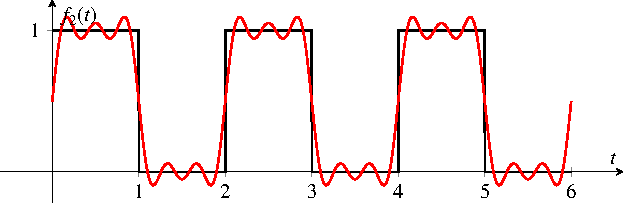
\includegraphics{papers/fourier/images/fourier_Rechteck.pdf}
	\caption{Fourierapproximation einer Rechteckfunktion, bei der in der Nähe der Sprungstellen das Gibbs-Phänomen auftritt.%
	\label{fourier:fig:fourierrechteck}}
\end{figure}

\begin{equation}
	f_1(t) = \frac{1}{2} + \sum_{\substack{n=1 \\ n\ \text{ungerade}}}^{5} \frac{1}{\pi n^2} \sin\left( \pi n t \right)
\end{equation}

$f_1(t)$ entspricht der roten Funktion. 
Der Mittelwert $a_0$ entspricht $\frac{1}{2}$. 
Die Rechteck Funktion ist abzüglich $a_0$ eine ungerade Funktion, da gilt $f_1(t) = -f_1(t)$. 
Daher ist der gerade Anteil $a_n$ stets Null. 
Zudem wurde noch eine vereinfachung von $b_n$ vorgenommen, da der Term bei geraden $n$ Null wird, summiert man nur über ungerade $n$. 


%
% fig-strahlungsspektren.tex
%
% (c) 2025 Prof Dr Andreas Müller
%
\begin{figure}
	\centering
	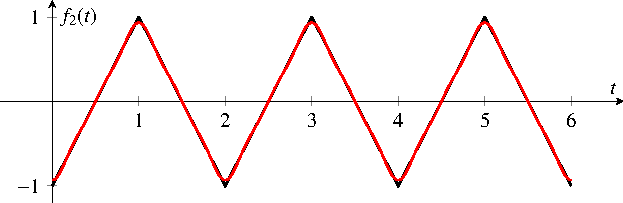
\includegraphics{papers/fourier/images/fourier_Dreieck.pdf}
	\caption{Fourierapproximation einer Dreieckfunktion}
	\label{fourier:fig:fourierdreieck}
\end{figure}


\begin{equation}
	f_2(t) = \sum_{\substack{n=1 \\ n\ \text{ungerade}}}^{5} \frac{8}{\pi^2 n^2} \cos(n\pi t)
\end{equation}

$f_2(t)$ entspricht der roten Funktion und überdeckt das Orginal beinahe perfekt. 
Dies mit nur drei Iterationen!
Der Mittelwert ist $a_0$ ist hier 0. 
Die Dreieck Funktion ist eine gerade Funktion, da gilt $f_1(t) = f_1(-t)$. 
Daher ist der ungerade Anteil $a_n$ stets Null. 
Wie beim ersten Beispiel wurde $b_n$ vereinfacht, man summiert nur über ungerade $n$. 


Bei der Fourier-Reihen Bildung kann man sich viel Zeit erspaaren, wenn man zuerst überprüft ob es sich um eine gerade oder ungerade Funktion handelt.
So kann man ohne zu rechnen $a_n$ oder $b_n$ gleich Null setzen.

%bei der Quantenmechanik rechnet man stets komplex. maybe noch erwähnen: die komplexe Fourierreihe



